\documentclass[12pt]{beamer}
\usepackage{../Estilos/BeamerFC}
\usepackage{../Estilos/ColoresLatex}
\input{../Preambulos/pre_codigo}
\input{../Preambulos/preambulo_Beamer_Warsaw_seahorse}
\usefonttheme{serif}

\title{Tema 0 - Introducción a python 2}
\author{M. en C. Gustavo Contreras Mayén}
\date{16 de agosto de 2022}

\begin{document}

\maketitle

\section*{Contenido}
\frame[allowframebreaks]{\tableofcontents[currentsection, hideallsubsections]}

\section{Colecciones}
\frame{\tableofcontents[currentsection, hideothersubsections]}
\subsection{Definición}

\begin{frame}
\frametitle{¿Qué es una colección?}
Hemos revisado algunos tipos de datos básicos en \python: números, booleanos y cadenas de texto.
\\
\bigskip
\pause
Ahora presentaremos los tipos de colecciones que se manejan en este lenguaje:
\pause
\setbeamercolor{item projected}{bg=tangerine,fg=black}
\setbeamertemplate{enumerate items}{%
\usebeamercolor[bg]{item projected}%
\raisebox{1.5pt}{\colorbox{bg}{\color{fg}\footnotesize\insertenumlabel}}%
}
\begin{enumerate}[<+->]
\item Listas.
\item Tuplas.
\item Diccionarios.
\end{enumerate}
\end{frame}

\subsection{Listas}

\begin{frame}
\frametitle{Las listas en \python}
Las listas son el tipo de dato más versátil de los datos compuestos de \python.
\\
\bigskip
Una lista contiene elementos separados por comas y entre corchetes $[ \quad ]$.
\end{frame}
\begin{frame}
\frametitle{Las listas en \python}
En cierta medida, las listas son similares a los arreglos (arrays) o vectores.
\\
\bigskip
Un punto importante de las listas: \pause es que \textbf{todos los elementos pertenecientes a una lista pueden ser de tipo de datos diferente}.
\end{frame}
\begin{frame}[fragile]
\frametitle{Ejemplos con listas}
Para introducir una lista, abrimos corchetes y separamos mediante comas los elementos de la misma:
\pause
\begin{lstlisting}[caption=Definiendo dos listas]
lista1 = ['abcd', 786, 2.23, 'salmon', 70.2]

lista2 = [ 123, 'pizza']

print(lista1)
print(lista2)
\end{lstlisting}
\end{frame}

\begin{frame}
\frametitle{Las listas en \python}
Los valores almacenados en una lista se recuperan usando la misma técnica de \emph{slicing} que vimos con las cadenas: \pause $[ \: ]$ y $[:]$, \pause donde los índices van desde  $0$ hasta el   $n - 1$.
\end{frame}
\begin{frame}[fragile]
\frametitle{Manejando las listas}
\begin{lstlisting}[caption=Usando el slicing en una lista]
print(lista1[2:])
print()
print(lista1[-1])
print()
print(lista1[2:4])
\end{lstlisting}
\end{frame}
\begin{frame}[fragile]
\frametitle{Operaciones con las listas 2}
También se ocupan las operaciones de \emph{concatenación} ($+$) \pause y repetición en las listas ($*$):
\pause
\begin{lstlisting}[caption=Concatenación y repetición de listas]
print(lista1 + lista2)
print()
print(lista2*2)
\end{lstlisting}
\pause
Toma en cuenta que el resultado permanece en la memoria de la computadora hasta que se cierre el programa, no se está asignando a una variable.
\end{frame}
\begin{frame}[fragile]
\frametitle{Agregar elementos a una lista}
Las listas en \python{} son los únicos objetos en los que podemos agregar nuevos elementos (son \textbf{mutables}), para ello hay que utilizar la función \textoazul{append}:
\pause
\begin{lstlisting}[caption=Agregando un elemento a la lista]
lista1.append(654.321)
print(lista1)
\end{lstlisting}
\pause
El nuevo elemento ocupa el último lugar dentro de la lista.
\end{frame}
\begin{frame}[fragile]
\frametitle{Reemplazo de un elemento de la lista}
Con una lista en \python{} se puede reemplazar el contenido específico de un elemento, haciendo referencia al índice en particular:
\pause
\begin{lstlisting}[caption=Modificando el contenido de un elemento de la lista]
print(lista2)
lista2[1] = 'coordenada'
print()
print(lista2)
\end{lstlisting}
\end{frame}
\begin{frame}[fragile]
\frametitle{Característica de las listas}
Las listas son un tipo de objeto en \python{} que permite que dentro de la misma, pueda contener a su vez, otra lista:
\pause
\begin{lstlisting}[caption=Una lista dentro de una lista]
print(lista1)
lista1.append(lista2)
print()
print(lista1)
\end{lstlisting}
\end{frame}

\subsection{Tuplas}

\begin{frame}
\frametitle{Las tuplas en \python}
Una tupla es otro tipo de datos de secuencia que es similar a la lista.
\\
\bigskip
\pause
Una tupla consiste en un grupo de valores separados por comas, identificamos a una tupla por que ésta usa paréntesis $( \quad )$.
\end{frame}
\begin{frame}
\frametitle{Característica de las tuplas}
Las principales características de las tuplas son:
\pause
\setbeamercolor{item projected}{bg=airforceblue,fg=aliceblue}
\setbeamertemplate{enumerate items}{%
\usebeamercolor[bg]{item projected}%
\raisebox{1.5pt}{\colorbox{bg}{\color{fg}\footnotesize\insertenumlabel}}%
}
\begin{enumerate}[<+->]
\item Los elementos de las tuplas no pueden modificarse (son \textbf{inmutables}).
\item No es posible agregar nuevos elementos a un tupla.
\item No podemos modificar el contenido de los elementos de la tupla.
\item Identificamos lo que una tupla contiene mediante el manejo de índices: usando el \emph{slicing}.
\end{enumerate}
\pause
Las tuplas pueden ser consideradas como listas de sólo lectura.
\end{frame}
\begin{frame}[fragile]
\frametitle{Ejemplos con tuplas}
\begin{lstlisting}[caption=Definiendo tuplas]
tupla1 = ('abcd', 786, 2.23, 'arena', 70.2)
tupla2 = (3.14, 'playa')

print(tupla1)
print()
print(tupla2)
print()
print(type(tupla1))
\end{lstlisting}
\end{frame}
\begin{frame}[fragile]
\frametitle{Manejando las tuplas}
Podemos seleccionar los elementos de la tupla mediante el uso de índices de contenido:
\pause
\begin{lstlisting}[caption=Recuperando elementos de una tupla]
print(tupla1[0])
print()
print(tupla1[-1])
\end{lstlisting}
\end{frame}
\begin{frame}[fragile]
\frametitle{Manejando las tuplas}
Podemos seleccionar los elementos de la tupla mediante el uso de \emph{slicing}:
\pause
\begin{lstlisting}[caption=Recuperando elementos de una tupla]
print(tupla1[1:3])
print()
print(tupla1[2:5])
\end{lstlisting}
\pause
\textbf{¿Por qué no tenemos un error al indicar un índice que no corresponde a la tupla?}
\end{frame}
\begin{frame}[fragile]
\frametitle{Errores con el manejo de tuplas}
Si queremos modificar el contenido de una tupla, obtendremos un mensaje de error:
\pause
\begin{lstlisting}[caption=Intentando modificar una tupla]
tupla1[2] = 'hola'
\end{lstlisting}
\end{frame}
\begin{frame}[fragile]
\frametitle{Errores con el manejo de tuplas}    
\begingroup
\fontsize{10}{10}\selectfont
\begin{verbatim}
TypeError     Traceback (most recent call last)

<stdin> in <module>()
----> 1 tupla1[2] = 'hola'

TypeError: 'tuple' object does not support
 item assignment
\end{verbatim}
\endgroup
\end{frame}
\begin{frame}[fragile]
\frametitle{Errores con el manejo de tuplas}
Si queremos agregar un elemento a la tupla, obtendremos un mensaje de error:
\pause
\begin{lstlisting}[caption=Intentando agregar un nuevo elemento a la tupla]
tupla1.append(100.56)
\end{lstlisting}
\end{frame}
\begin{frame}[fragile]
\frametitle{Errores con el manejo de tuplas}    
\begingroup
\fontsize{10}{10}\selectfont
\begin{verbatim}
TypeError     Traceback (most recent call last)

<stdin> in <module>()
----> 1 tupla1.append(100.56)

AttributeError: 'tuple' object has no 
  attribute 'append'
\end{verbatim}
\endgroup
\end{frame}

\subsection{Diccionarios}

\begin{frame}
\frametitle{Diccionarios}
Los diccionarios de \python{} son de tipo tabla-hash.
\\
\bigskip
\pause
Funcionan como matrices asociativas y consisten en pares \emph{\textcolor{cadmiumred}{llave} - \textcolor{cadmiumgreen}{valor}}.
\end{frame}
\begin{frame}
\frametitle{Elementos del diccinario}
La \emph{\textcolor{cadmiumred}{llave}} del diccionario puede ser casi de cualquier tipo de dato, pero suelen ser comúnmente números o cadenas.
\\
\bigskip
\pause
El \textcolor{cadmiumgreen}{valor}, por otra parte, puede ser cualquier tipo de objeto arbitrario de \python.
\end{frame}
\begin{frame}[fragile]
\frametitle{Escribir un diccionario}
Para crear un diccionario se debe de iniciar con las llaves $\{ \quad \}$, \pause el siguiente valor corresponde a la llave seguida de dos puntos y a continuación, el valor:
\\
\bigskip
\pause
\begin{align*}
\mbox{mi\_dict } = \{ \mbox{'valor1'} : \mbox{'llave1'}, \mbox{'valor2'} : \mbox{'llave2'} , \ldots \} 
\end{align*}
\end{frame}
\begin{frame}[fragile]
\frametitle{Escribir un diccionario}
La siguiente instrucción se escribe en una sola línea:
\pause
\begin{lstlisting}[caption=Escribiendo un diccionario]
fisicos = {1 : "Eistein", 2 : "Bohr", 
3 : "Pauli", 4 : "Schrodinger", 
5 : "Hawking"}

print(fisicos)
\end{lstlisting}
\end{frame}
\begin{frame}[fragile]
\frametitle{Recuperando los elementos de un diccionario}
Hay un conjunto de funciones que nos permiten recuperar tanto las llaves como los valores de un diccionario:
\pause
\begin{lstlisting}[caption=Recuperando el contenido de un diccionario]
fisicos.keys()

fisicos.values()
\end{lstlisting}
\end{frame}
\begin{frame}[fragile]
\frametitle{Agregar un nuevo elemento al diccionario}
Es posible agregar un nuevo elemento al diccionario con la siguiente función:
\pause
\begin{lstlisting}[caption=Agregando un elemento al diccionario]
print(fisicos)

fisicos.update({6:'Dirac'})
print()
print(fisicos)
\end{lstlisting}
\pause
Recordemos que este cambio solo queda en memoria, ya que no se ha asignado a una variable.
\end{frame}

\section{Identificadores en python}
\frame{\tableofcontents[currentsection, hideothersubsections]}
\subsection{Reglas para los identificadores}

\begin{frame}
\frametitle{Reglas para los identificadores}
Los identificadores son nombres que hacen referencia a los objetos que componen un programa: \textbf{constantes}, \textbf{variables}, \textbf{funciones}, \textbf{módulos}, \textbf{clases} etc.
\end{frame}
\begin{frame}
\frametitle{Reglas para los identificadores}
Se recomienda seguir las reglas para construir identificadores:
\begin{itemize}[<+->]
\item[\ding{212}] El primer carácter debe ser una letra o el carácter de subrayado (guión bajo)
\item[\ding{212}] El primer carácter puede ir seguido de un número variable de dígitos numéricos, letras o carácteres de subrayado.
\end{itemize}
\end{frame}
\begin{frame}
\frametitle{Reglas para los identificadores}
\begin{itemize}[<+->]
\item[\ding{212}] No pueden utilizarse espacios en blanco, ni símbolos de puntuación.
\item[\ding{212}] En \python{} se distingue de las mayúsculas y minúsculas.
\end{itemize}
\end{frame}
\begin{frame}
\frametitle{Reglas para los identificadores}
Existe un estándar para la escritura del código en \python, revisa en la siguiente liga, el manejo de los nombres de los identificadores en: \href{shorturl.at/fOUV7}{\color{blue}{\underline{Referencia para nombres de objetos en \python{}}}}, del estándar PEP-8.
\end{frame}
\begin{frame}
\frametitle{Palabras reservadas}
No pueden utilizarse las palabras reservadas de \python{} para ningún tipo de identificador, \pause ya que son palabras reservadas para la ejecución de comandos, funciones, tareas, etc. propias de \python{} (de igual manera que son reservadas en otros lenguajes de programación o del mismo sistema operativo), entre las más comunes tenemos:
\end{frame}
\begin{frame}
\frametitle{Palabras reservadas}
\texttt{
\fontsize{12}{12}\selectfont
\begin{table}
\begin{tabular}{c c c c c }
del & for & is & raise & assert \\ \hline
elif & global & else & or & yield  \\ \hline
from & lamda & return & break & system \\ \hline
not & try & class & except & if \\ \hline
while & continue & exec & import & pass \\ \hline
def & finally & in & print & del \\ \hline
\end{tabular}
\end{table}
}
\end{frame}

\section{Estructuras de control}
\frame{\tableofcontents[currentsection, hideothersubsections]}
\subsection{¿Qué son las estructuras de control?}

\begin{frame}
\frametitle{Estructuras de control}
En cualquier lenguaje de programación se incluye una serie de estructuras de control para ampliar el control, la lógica y ejecución de un programa.
\\
\bigskip
En \python, manejaremos las más comunes, que son relativamente sencillas de usar, cuidado siempre la sintaxis respectiva.
\end{frame}
\begin{frame}
\frametitle{Las estructuras de control}
Revisaremos las siguientes estructuras:
\setbeamercolor{item projected}{bg=darkbrown,fg=cream}
\setbeamertemplate{enumerate items}{%
\usebeamercolor[bg]{item projected}%
\raisebox{1.5pt}{\colorbox{bg}{\color{fg}\footnotesize\insertenumlabel}}%
}
\begin{enumerate}[<+->]
\item Condicionales.
\item  Bucles (iterativas).
\end{enumerate}
\end{frame}

\section{Condicionales}
\frame[allowframebreaks]{\tableofcontents[currentsection, hideothersubsections]}
\subsection{¿Qué es un condicional?}

\begin{frame}
\frametitle{Los condicionales}
Una estructura condicional inicialmente evalúa si una o más condiciones cumplen con un valor \textoazul{\texttt{True}}.
\\
\bigskip
\pause
Si la condición (o condiciones) se cumplen, entonces pasa a un bloque de instrucciones que se van a ejecutar.
\end{frame}
\begin{frame}
\frametitle{Los condicionales}    
En caso de que el valor de la condición (o condiciones) no se cumpla, \pause es decir, tienen un valor \textcolor{red}{\texttt{False}}, \pause no se pasa al bloque con las instrucciones contenidas.
\\
\bigskip
\pause
Se ejecuta la siguiente línea de código fuera del condicional.
\end{frame}

\subsection{El condicional if}

\begin{frame}[fragile]
\frametitle{El condicional if}
El condicional \funcionazul{if} requiere de una expresión inicial que va a evaluar, como ya se mencionó, en caso de que no se cumpla el valor \textoazul{\texttt{True}}, no se ejecutan las instrucciones contenidas.
\begin{verbatim}
if expresion:
    instruccion1
    instruccion2

siguiente línea código
\end{verbatim}
\end{frame}
\begin{frame}[fragile]
\frametitle{Ejemplo de condicional if}
El siguiente ejemplo es un condicional \textoazul{if}:
\pause
\begin{lstlisting}[caption=La estructura condicional if]
distancia = 100
tiempo = 60

if distancia < 1000:
    print('La distancia es menor a un kilómetro')

print(distancia/tiempo)
\end{lstlisting}
\end{frame}

\subsection{El condicional if-else}

\begin{frame}
\frametitle{El condicional if-else:}
Cuando tenemos un condicional con \funcionazul{if} y la expresión que se evalúa tiene un valor \textcolor{red}{False}, sabemos que saldrá del bloque condicional.
\\
\bigskip
\pause
Pero si queremos que se ejecute otro bloque de instrucciones a pesar de que al inicio la expresión evaluada sea \textcolor{red}{False}, \pause recurrimos a la instrucción \funcionazul{else:}, por lo que se ejecutan las instrucciones contenidas dentro de este bloque.
\end{frame}
\begin{frame}[fragile]
\frametitle{El condicional \texttt{if-else:}}
\begin{verbatim}
if expresion1:
    instruccion1
    instruccion2
else:
    instruccion-else-1
    instruccion-else-2

siguiente línea código
\end{verbatim}
\end{frame}
\begin{frame}[fragile]
\frametitle{Ejemplo de condicional if-else}
\begin{lstlisting}[caption=La estructura condicional if-else]
distancia = 1500
tiempo = 60

if distancia < 1000:
    print('La distancia es menor a un kilómetro')
else:
    print('La distancia es mayor a un kilómetro')

print('La velocidad es: ', distancia/tiempo)
\end{lstlisting}
\end{frame}

\subsection{El condicional if-elif}

\begin{frame}[fragile]
\frametitle{El condicional \texttt{if-elif:}}
El condicional \funcionazul{if} evalúa al inicio solo una expresión (o expresiones), \pause en ocasiones se puede incluir la evaluación de una segunda expresión distinta mediante:
\end{frame}
\begin{frame}[fragile]
\frametitle{El condicional \texttt{if-elif:}}
\begin{verbatim}
if expresion1:
    instruccion1
    instruccion2
elif expresion2:
    otra-instruccion1
    otra-instruccion2

siguiente línea código
\end{verbatim}
\end{frame}
\begin{frame}
\frametitle{El condicional \texttt{if-elif:}}
La \texttt{expresion1} no se cumple, por lo que se pasa a la siguiente línea.
\\
\bigskip
\pause
Si \texttt{expresion2} devuelve un valor \textoazul{\texttt{True}}, entonces se ejecutan las instrucciones contenidas en ese bloque.
\end{frame}
\begin{frame}[fragile]
\frametitle{Ejemplo de condicional if-elif}
\begin{lstlisting}[caption=La estructura condicional if-elif]
distancia = 1500

if distancia <= 1000:
    print('La distancia es menor a un kilómetro')
elif distancia <= 2000:
    print('La distancia es menor a dos kilómetros')
\end{lstlisting}
\end{frame}    

\subsection{El condicional if-elif-else}

\begin{frame}[fragile]
\frametitle{El condicional \texttt{if-elif-else:}}
Podemos ocupar en condicional \texttt{if-elif:} en donde se evalúan dos expresiones, en caso de que ambas sean \textcolor{red}{False}, se ejecuta el código contenido en \funcionazul{else:}
\end{frame}
\begin{frame}[fragile]
\frametitle{El condicional \texttt{if-elif-else:}}
\fontsize{12}{12}\selectfont
\begin{verbatim}
if expresion1:
    instruccion1
    instruccion2
elif expresion2:
    instruccion-elif-1
    instruccion-elif-2
else:
    instruccion-else-1
    instruccion-else-2

siguiente línea código
\end{verbatim}
\end{frame}
\begin{frame}[fragile]
\frametitle{Ejemplo de condicional \texttt{if-elif-else:}}
\begin{lstlisting}[caption=Ejemplo de un condicionla if-elif-else]
a = int(input('Introduce el valor de a'))
if a > 0:
    print ("a es positivo")
    a = a + 1
elif a == 0: 
    print ("a es 0")
else:
    print ("a es negativo")
\end{lstlisting}
\end{frame}
\begin{frame}
\frametitle{La función \texttt{input}}
En el ejemplo anterior la función \funcionazul{input}, permite el ingreso de datos por parte del usuario.
\\
\bigskip
\pause
Todo aquel valor que se introduce, se toma como una \emph{cadena}, por ello se utiliza la función \funcionazul{int ()} para convertirla a un tipo de dato entero.
\end{frame}

\subsection{Bucles o Loops}

\begin{frame}
\frametitle{Bucles}
Un bucle es una sentencia que ejecuta un mismo conjunto de instrucciones, de manera repetida mientras se satisface una condición.
\\
\bigskip
Se evalúa inicialmente una condición, en caso de que su valor sea (valor \funcionazul{True}) se ejecutan las instrucciones contenidas, \pause la estructura termina al cambiar el valor de la condición.
\end{frame}
\begin{frame}
\frametitle{Las estructuras de bucle}
En \python{} se tienen dos estructuras iterativas:
\setbeamercolor{item projected}{bg=aqua,fg=ao}
\setbeamertemplate{enumerate items}{%
\usebeamercolor[bg]{item projected}%
\raisebox{1.5pt}{\colorbox{bg}{\color{fg}\footnotesize\insertenumlabel}}%
}
\begin{enumerate}[<+->]
\item \funcionazul{for-in}
\item \funcionazul{while}
\end{enumerate}
\end{frame}

\subsection*{Sentancia \texttt{for ... in}}

\begin{frame}
\frametitle{Sentencia for ... in}
Es una forma genérica de iterar sobre una secuencia.
\\
\bigskip
\pause
Podemos usar como secuencia: \pause tanto \emph{listas} como \emph{tuplas} o generar una, para ejecutar el bucle un número determinado de veces.
\end{frame}
\begin{frame}[fragile]
\frametitle{Ejemplo del bucle \texttt{for-in}}
Usaremos un objeto lista y el ciclo \funcionazul{for-in}:
\pause
\begin{lstlisting}[caption=Ejemplo del ciclo for-in]
alfabeto = ["alfa", "beta", "gama", "delta"]
for letra in alfabeto:
    print (letra)
\end{lstlisting}
\end{frame}
\begin{frame}[fragile]
\frametitle{Ejemplo del bucle \texttt{for-in}}
En este ejemplo la instrucción \funcionazul{print} se ejecutará tantas veces como elementos haya en la lista \emph{alfabeto}, en cada iteración la variable \emph{letra} tomará el valor de cada uno de los elementos de la lista.
\end{frame}
\begin{frame}
\frametitle{Iteración sobre secuencia de números}
¿Cómo le hacemos para iterar sobre una serie de números naturales consecutivos? \pause Por ejemplo del $1$ al $20$.
\\
\bigskip
\pause
 Para ello usaremos la función \funcionazul{range(\ )}. Esta función genera una lista con una progresión aritmética de números naturales.
 \end{frame}
\begin{frame}
\frametitle{Argumentos de la función \texttt{range}}
\setbeamercolor{item projected}{bg=armygreen,fg=aquamarine}
\setbeamertemplate{enumerate items}{%
\usebeamercolor[bg]{item projected}%
\raisebox{1.5pt}{\colorbox{bg}{\color{fg}\footnotesize\insertenumlabel}}%
}
\begin{enumerate}[<+->]
\item Si le pasamos un único parámetro se generará una lista que va desde $0$ hasta $n-1$.
\pause
\begin{align*}
\mbox{range} (10)
\end{align*}
\seti
\end{enumerate}  
\end{frame}
\begin{frame}
\frametitle{Argumentos de la función \texttt{range}}
\setbeamercolor{item projected}{bg=armygreen,fg=aquamarine}
\setbeamertemplate{enumerate items}{%
\usebeamercolor[bg]{item projected}%
\raisebox{1.5pt}{\colorbox{bg}{\color{fg}\footnotesize\insertenumlabel}}%
}
\begin{enumerate}[<+->]
\conti    
\item Si le damos dos argumentos: \funcionazul{(inicio, fin)}, generará una lista desde \textoazul{inicio} hasta \textoazul{fin - 1}.
\pause
\begin{align*}
\mbox{range} (1, 10)
\end{align*}
\seti
\end{enumerate}  
\end{frame}
\begin{frame}
\frametitle{Argumentos de la función \texttt{range}}
\setbeamercolor{item projected}{bg=armygreen,fg=aquamarine}
\setbeamertemplate{enumerate items}{%
\usebeamercolor[bg]{item projected}%
\raisebox{1.5pt}{\colorbox{bg}{\color{fg}\footnotesize\insertenumlabel}}%
}
\begin{enumerate}[<+->]
\conti
\item Si le damos tres argumentos: \break \hfill \funcionazul{(inicio, fin, paso)}, usará el \textoazul{paso} como incremento para generar los elementos de la lista.
\pause
\begin{align*}
\mbox{range} (1, 20, 3)
\end{align*}    
\end{enumerate}  
\end{frame}
\begin{frame}[fragile]
\frametitle{Ejemplos del bucle \texttt{for-in}}
\begin{lstlisting}[caption=Ejemplos con varios parámetros en la función range]
print(list(range(10)))
print()
print(list(range(1, 10)))
print()
print(list(range(1, 20, 3)))
\end{lstlisting}
\end{frame}
\begin{frame}[fragile]
\frametitle{Recorriendo los elementos de una cadena}
Podemos usar una cadena de caracteres como secuencia, de forma que en cada iteración se tomará un elemento de la cadena.
\pause
\begin{lstlisting}[caption=Recorriendo una cadena]
for letra in 'ABCD':
    print(letra)
\end{lstlisting}
\end{frame}
\begin{frame}[fragile]
\frametitle{Recorriendo una lista con \texttt{enumerate}}
En caso de que necesitemos iterar sobre una \emph{lista} y a la vez recuperar el índice de cada elemento de la lista, \pause usaremos la función \funcionazul{enumerate( )} que devuelve dos valores: la \textcolor{darkgreen}{índice} y el \textcolor{lava}{elemento} de la lista.
\pause
\begin{lstlisting}[caption=Recorriendo con índices y elementos de una lista]
figura = ["recta", "círculo", "cono", "plano", "esfera"]
for indice, elemento in enumerate(figura):
    print(indice, elemento)
\end{lstlisting}
\end{frame}

\subsection{Sentencia \texttt{while}}

\begin{frame}
\frametitle{La sentencia \texttt{while}}
Ese bucle repite un conjunto de instrucciones mientras se cumpla una determinada condición que se evalúa al principio de cada ejecución.
\end{frame}
\begin{frame}[fragile]
\frametitle{La sentencia \texttt{while}}
\fontsize{12}{12}\selectfont
\begin{verbatim}
while expresion:
    instruccion1
    instruccion2
    ...

siguiente línea código
\end{verbatim}
\end{frame}
\begin{frame}[fragile]
\frametitle{Ejemplo de una sentencia \texttt{while}}
\begin{lstlisting}[caption=Primer ejemplo de un ciclo while]
angulo = 30

while angulo <= 42:
    print(angulo)
    angulo = angulo + 1
\end{lstlisting}
\end{frame}
\begin{frame}
\frametitle{Ciclo \texttt{while} infinito}
Es evidente que las instrucciones dentro del bucle \textoazul{while} tendrán que hacer algo que cambie el valor de la condición, para que termine la sentencia.
\\
\bigskip
En caso contrario tendremos un \textcolor{brickred}{bucle infinito} y el programa nunca terminará su ejecución.
\end{frame}
\begin{frame}
\frametitle{Repeticiones en el ciclo \texttt{while}}
Una de las características del bucle \funcionazul{while} es que no está fijado previamente el número de veces que se ejecutan las instrucciones del bucle.
\\
\bigskip
Se ejecutarán todas las que sean necesarias mientras se cumpla la condición.
\end{frame}
\begin{frame}
\frametitle{Forzar la salida del bucle \texttt{while}}
Como hemos mencionado, la sentencia \funcionazul{while} va a iterar mientras se cumpla una condición.
\\
\bigskip
Pero vamos a encontrar que en ocasiones, necesitamos \enquote{salir} del bucle sin que tengamos que esperar a que la condición cambie.
\end{frame}
\begin{frame}[fragile]
\frametitle{Forzar la salida del bucle \texttt{while}}
Hay dos palabras reservadas que se usan dentro de un bucle \texttt{while}:
\pause
\setbeamercolor{item projected}{bg=bronze,fg=bubbles}
\setbeamertemplate{enumerate items}{%
\usebeamercolor[bg]{item projected}%
\raisebox{1.5pt}{\colorbox{bg}{\color{fg}\footnotesize\insertenumlabel}}%
}
\begin{enumerate}[<+->]
\item \funcionazul{continue}.
\item \funcionazul{break}.
\end{enumerate}
\end{frame}
\begin{frame}[fragile]
\frametitle{Forzar la salida con \texttt{continue}}
Con \funcionazul{continue} pasamos de nuevo al principio del bucle, aunque no se haya terminado de ejecutar el ciclo.
\begin{lstlisting}
edad = 0
while edad < 18:
    edad = edad + 1
    if edad % 2 == 0:
        continue
    print ("Felicidades, tienes " + str(edad))
\end{lstlisting}
\end{frame}
\begin{frame}[fragile]
\frametitle{Forzar la salida con \texttt{break}}
Por su parte, \funcionazul{break} hace que salgamos del bucle \funcionazul{while} directamente sin necesidad de volver a evaluar la condición, aunque siga siendo cierta.
\end{frame}
\begin{frame}[fragile]
\frametitle{Forzar la salida con \texttt{break}}
\begin{lstlisting}[caption=Forzando la salida del bucle con break]
while True:
    entrada = input("> ")
    if entrada == "adios":
        break
    else:
        print (entrada)
\end{lstlisting}
\end{frame}

\section{Manejo de excepciones}
\frame{\tableofcontents[currentsection, hideothersubsections]}
\subsection{Tipos de errores}

\begin{frame}[fragile]
\frametitle{Manejo de excepciones}
Cuando comenzamos a programar, nos podemos encontrar con mensajes de error al momento de ejecutar el programa, siendo las causas más comunes:
\pause
\setbeamercolor{item projected}{bg=burgundy,fg=buff}
\setbeamertemplate{enumerate items}{%
\usebeamercolor[bg]{item projected}%
\raisebox{1.5pt}{\colorbox{bg}{\color{fg}\footnotesize\insertenumlabel}}%
}
\begin{enumerate}[<+->]
\item Errores de dedo: escribiendo incorrectamente una instrucción, sentencia, variable o constante.
\item Errores al momento de introducir los datos, por ejemplo, si el valor que se debe de ingresar es $123.45$, y si nosotros tecleamos $1234.5$, el resultado ya se considera un error.
\seti
\end{enumerate}
\end{frame}
\begin{frame}[fragile]
\frametitle{Manejo de excepciones}
\setbeamercolor{item projected}{bg=burgundy,fg=buff}
\setbeamertemplate{enumerate items}{%
\usebeamercolor[bg]{item projected}%
\raisebox{1.5pt}{\colorbox{bg}{\color{fg}\footnotesize\insertenumlabel}}%
}
\begin{enumerate}[<+->]
\conti    
\item Errores que se muestran en tiempo de ejecución, es decir, todo está bien escrito y los datos están bien introducidos, pero hay un error debido a la lógica del programa o del método utilizado, ejemplo: división entre cero.
\end{enumerate}
\end{frame}
\begin{frame}
\frametitle{El programa se detiene con un error}
Cuando se presenta un error en la ejecución del código, el programa se detiene.
\\
\bigskip
\pause
Siendo necesario corregir el error y nuevamente, ejecutar el programa.
\end{frame}
\begin{frame}[fragile]
\frametitle{Manejo de errores}
En el siguiente ejemplo, obtendremos de antemano un error por intentar una operación matemática no permitida.
\\
\bigskip
\verb|c = 12.0/0.0| \\
\pause
%\begin{exampleblock}{}
\verb|Traceback (most recent call last):| \\
\verb|File ''<pyshell#0>'', line 1, in ?| \\
\verb|c = 12.0/0.0| \\
\verb|ZeroDivisionError: float division|
%\end{exampleblock}
\end{frame}
\begin{frame}[fragile]
\frametitle{Manejo de excepciones}
Veamos el siguiente ejemplo:
\begin{lstlisting}
while True print('Hola mundo')

  File "<stdin>", line 1
    while True print('Hola mundo')
                   ^
SyntaxError: invalid syntax
\end{lstlisting}
\end{frame}
\begin{frame}
\frametitle{Información del error}
\fontsize{13}{13}\selectfont
El intérprete de \python{} indica la línea \emph{culpable} y muestra una pequeña \enquote{marca} que apunta al lugar donde se detectó el error.
\\
\bigskip
Este es causado por (o al menos detectado en) el símbolo que precede a la flecha: en el ejemplo, el error se detecta en la función \azulfuerte{print()}, ya que faltan dos puntos \azulfuerte{(:)} antes del mismo.
\\
\bigskip
Se muestran el nombre del archivo y el número de línea para que sepas dónde mirar en caso de que la entrada venga de un programa.    
\end{frame}
\begin{frame}
\frametitle{Tipos de error en \python}
Es importante conocer los distintos tipos de error que pueden generarse en \python, en la documentación oficial podremos encontrar una lista con el nombre del tipo de error y por qué se genera.
\end{frame}
\begin{frame}
\frametitle{Errores aritméticos}
\setbeamercolor{item projected}{bg=charcoal,fg=champagne}
\setbeamertemplate{enumerate items}{%
\usebeamercolor[bg]{item projected}%
\raisebox{1.5pt}{\colorbox{bg}{\color{fg}\footnotesize\insertenumlabel}}%
}
\begin{enumerate}[<+->]
\item \funcionazul{OverflowError}
\item \funcionazul{ZeroDivisionError}
\item \funcionazul{FloatingPointError}
\end{enumerate}
\end{frame}
\begin{frame}
\frametitle{Errores generales}
\setbeamercolor{item projected}{bg=deeplilac,fg=deeppeach}
\setbeamertemplate{enumerate items}{%
\usebeamercolor[bg]{item projected}%
\raisebox{1.5pt}{\colorbox{bg}{\color{fg}\footnotesize\insertenumlabel}}%
}
\begin{enumerate}[<+->]
\item \funcionazul{ImportError}
\item \funcionazul{IndexError}
\item \funcionazul{KeyboardInterrupt}
\item \funcionazul{NameError}
\item \funcionazul{SyntaxError}
\item \funcionazul{TabError}
\item \funcionazul{ValueError}
\end{enumerate}
\end{frame}

\subsection{Creando un manejo de excepciones}

\begin{frame}
\frametitle{¿Qué es el manejo de excepciones?}
En programación se conoce como \textoazul{excepción} a un error que se detecta en ejecución.
\\
\bigskip
\pause
El manejo de excepciones es un código que las gestiona y que le permiten al usuario dar solución para que el programa continúe.
\end{frame}
\begin{frame}[fragile]
\frametitle{Estructura del manejo de excepciones}
\begin{figure}
    \centering
    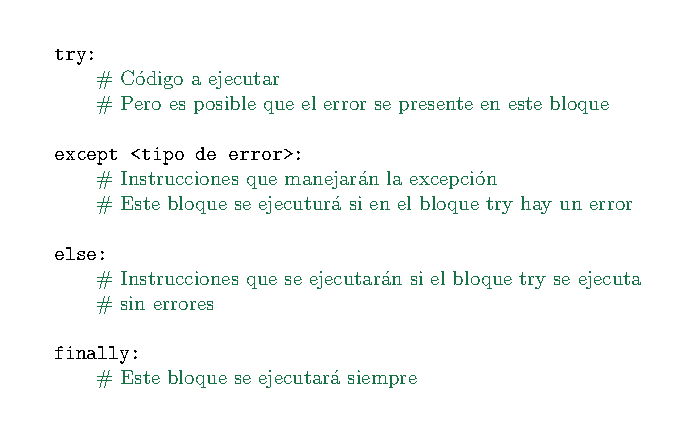
\includegraphics[scale=0.95]{Imagenes/Manejo_Excepciones_01.eps}
\end{figure}
\end{frame}
\begin{frame}[fragile]
\frametitle{Ejemplo de un manejo de excepción}
\begin{lstlisting}[caption=Un error por la variable x no definida]
try:
    print(x)
except NameError:
    print('La variable \'x\' no está definida')
except:
    print('Algo salió mal')
\end{lstlisting}
\end{frame}
\begin{frame}[fragile]
\frametitle{Otro ejemplo de un manejo de excepción}
\begin{lstlisting}[caption=Manejo con un else]
    try:
    print('Hola mundo!')
except:
    print('Algo salió mal')
else:
    print('No hubo problemas')
\end{lstlisting}
\end{frame}
\begin{frame}[fragile]
\frametitle{Otro ejemplo de un manejo de excepción}
\begin{lstlisting}[caption=Manejo con un else]
try:
    print('Hola mundo!')
except:
    print('Algo salió mal')
else:
    print('No hubo problemas')
finally:
    print('Salimos del manejo de excepciones')
\end{lstlisting}
\end{frame}
\begin{frame}
\frametitle{Generando excepciones propias}
Podemos generar una excepción si se produce una condición en particular.
\\
\bigskip
\pause
Para \enquote{lanzar} (o generar) una excepción, usamos la palabra clave \funcionazul{raise}.
\end{frame}
\begin{frame}[fragile]
\frametitle{Generando excepción por tipo de error}
Podems definir el tipo de error para generar la excepción y el texto que se le mostrará al usuario.
\begin{lstlisting}[caption=Generando una excepción]
x = 'Hola!'

if not type(x) is int:
    raise TypeError('Solo se permiten enteros')
\end{lstlisting}    
\end{frame}
\begin{frame}
\frametitle{Algunos tipos de error}
\setbeamercolor{item projected}{bg=dodgerblue,fg=eggshell}
\setbeamertemplate{enumerate items}{%
\usebeamercolor[bg]{item projected}%
\raisebox{1.5pt}{\colorbox{bg}{\color{fg}\footnotesize\insertenumlabel}}%
}
\begin{enumerate}[<+->]
\item \textoazul{ArtimethicError}: Errores aritméticos.
\item \textoazul{FloatingPointError}: Error en una operación de punto flotante.
\item \textoazul{OverflowError}: Resultado demasiado grande para representarlo.
\item \textoazul{ZeroDivisionError}: Cuando el segundo argumento de una división o módulo es $0$.
\item \textoazul{EOFError}: Se intentó leer más allá del final del archivo.
\item \textoazul{IOError}: Error en una operación de entrada/salida.
\end{enumerate}
\end{frame}
% \begin{frame}[fragile]
% \frametitle{Manejando excepciones}
% Es posible escribir programas que manejen determinadas excepciones. 
% \\
% \bigskip
% En el siguiente ejemplo, se le pide al usuario una entrada hasta que ingrese un entero válido, pero permite al usuario interrumpir el programa (usando \keys{\ctrl} + \keys{C}) o lo que sea que el sistema operativo soporte)
% \end{frame}
% \begin{frame}[fragile]
% \frametitle{Manejando excepciones}
% \begin{lstlisting}
% while True:
%     try:
%         x = int(input("Por favor ingrese un numero: "))
%         break
%     except ValueError:
%         print("Oops! No era valido. Intente nuevamente...")
% \end{lstlisting}
% \end{frame}
% \begin{frame}
% \frametitle{La declaración \texttt{try}}
% La declaración try funciona de la siguiente manera:
% \begin{itemize}[<+->]
% \item Primero, se ejecuta el bloque \azulfuerte{try} (el código entre las declaración \azulfuerte{try} y \azulfuerte{except}).
% \item  Si no ocurre ninguna excepción, el bloque \azulfuerte{except} se salta y termina la ejecución de la declaración \azulfuerte{try}.
% \end{itemize}
% \end{frame}
% \begin{frame}
% \frametitle{La declaración \texttt{try}}
% \begin{itemize}[<+->]
% \item  Si ocurre una excepción durante la ejecución del bloque \azulfuerte{try}, el resto del bloque se salta. Luego, si su tipo coincide con la excepción nombrada luego de la palabra reservada \azulfuerte{except}, se ejecuta el bloque \azulfuerte{except}, y la ejecución continúa luego de la declaración \azulfuerte{try}.
% \end{itemize}
% \end{frame}
% \begin{frame}
% \frametitle{La declaración \texttt{try}}
% \begin{itemize}[<+->]
% \item Si ocurre una excepción que no coincide con la excepción nombrada en el \azulfuerte{except}, esta se pasa a declaraciones \azulfuerte{try} de más afuera; si no se encuentra nada que la maneje, es una \emph{excepción no manejada}, y la ejecución se frena con un mensaje como los mostrados arriba.
% \end{itemize}
% \end{frame}
% \begin{frame}[fragile]
% \frametitle{Manejo de excepciones más elaborado}
% El siguiente código considera un manejo de excepciones por su tipo:
% \fontsize{12}{11}\selectfont
% \begin{verbatim}
% try:
%     <código suceptible de errores>
% except <ErrorTipo1>:
%     <bloque inscrito a ErrorTipo1>
% except< ErrorTipo2>:
%     <bloque inscrito a ErrorTipo2>
% except (<ErrorTipo3>, <ErrorTipo4>):
%     <bloque inscrito a ErrorTipo3 y ErrorTipo4>
% except:
%     <bloque inscrito a except general>
% \end{verbatim}
% \end{frame}
% \begin{frame}[fragile]
% \frametitle{Consideraciones sobre la gestión de excepciones}
% Con la inclusión de las excepciones hemos visto que el programa no se interrumpe cuando existe un error.
% \\
% \bigskip
% Es posible mostrar más información al usuario sobre el tipo de error, recordemos que habrá alguien que ocupe nuestro programa y al contar con más información, podrá resolver la situación.
% \end{frame}
% \begin{frame}[allowframebreaks, fragile]
% \frametitle{Ejemplo}
% Veamos el siguiente ejemplo (las dos diapositivas contienen el código:
% \fontsize{11}{10}\selectfont
% \begin{lstlisting}
% ocurre_error = False

% try:
%     numero = float(input('Introduce un numero: '))
%     print("La raiz cuadrada de numero %f es %f" % (numero, numero ** 0.5))

% except TypeError as descripcion:
%     ocurre_error = True
%     print("Ocurrio un error previsto:", descripcion)

% except:
%     ocurre_error = True
%     print("!No se que paso!")

% if ocurre_error:
%     print("Lastima.")
% else:
%     print("Buen dia.")
% \end{lstlisting}
% \end{frame}
% \begin{frame}[fragile]
% \frametitle{Ejecutando el código}
% Ahora introducimos algunos valores para revisar la operación del código:
% \\
% \bigskip
% \pause
% \verb|Introduce un numero: 12|
% \\
% \pause
% \begin{lstlisting}
% La raiz cuadrada del numero 12.000000 es 3.464102
% Buen dia.
% \end{lstlisting}
% \end{frame}
% \begin{frame}[fragile]
% \frametitle{Ejecutando el código}
% Ahora introducimos un valor que provocará un error:
% \\
% \bigskip
% \pause
% \verb|Introduce un numero: -6|
% \\
% \pause
% \begin{lstlisting}
% Ocurrio un error previsto: can't convert complex to float
% Lastima.
% \end{lstlisting}
% \end{frame}
% \begin{frame}[fragile]
% \frametitle{Ejecutando el código}
% Ejecutamos nuevamente el código e introducimos un valor que provocará un error:
% \\
% \bigskip
% \pause
% \verb|Introduce un numero: q|
% \\
% \pause
% \begin{verbatim}
% No se que paso
% Lastima.
% \end{verbatim}
% \end{frame}
% \begin{frame}
% \frametitle{Explicación del resultado}
% Cuando se introdujo un número negativo $(-1)$, sabíamos que se presentaría un \textcolor{red}{TypeError} ya que no se puede evaluar la raíz cuadrada de un número negativo.
% \\
% \bigskip
% \pause
% Este tipo de error coincide con el señalado en la sentencia \funcionazul{except}, por lo que se muestra la descripción del error a modo de mensaje.
% \end{frame}
% \begin{frame}
% \frametitle{Explicación del resultado}
% Mientras que al introducir un caracter (q), el tipo de error no corresponde con \textcolor{red}{TypeError}, por lo que no \enquote{entra} en la primera sentencia \funcionazul{except} y pasa a la siguiente sentencia \funcionazul{except} de tipo general.
% \end{frame}


\end{document}